%%%%%%%%%%%%%%%%%%%%%%%%%%%%%%%%%%%%%%%%%%%%%%%%%%%%%%%%%%%%%%%%%%%%%%%%%%%%%%%%
%2345678901234567890123456789012345678901234567890123456789012345678901234567890
%        1         2         3         4         5         6         7         8

\documentclass[letterpaper, 10 pt, conference]{ieeeconf}  % Comment this line out if you need a4paper

%\documentclass[a4paper, 10pt, conference]{ieeeconf}      % Use this line for a4 paper
\usepackage{graphicx}
\usepackage{amsmath}
\usepackage{float}
\IEEEoverridecommandlockouts                              % This command is only needed if 
                                                          % you want to use the \thanks command

\overrideIEEEmargins                                      % Needed to meet printer requirements.

% See the \addtolength command later in the file to balance the column lengths
% on the last page of the document

% The following packages can be found on http:\\www.ctan.org
%\usepackage{graphics} % for pdf, bitmapped graphics files
%\usepackage{epsfig} % for postscript graphics files
%\usepackage{mathptmx} % assumes new font selection scheme installed
%\usepackage{times} % assumes new font selection scheme installed
%\usepackage{amsmath} % assumes amsmath package installed
%\usepackage{amssymb}  % assumes amsmath package installed

\title{\LARGE \bf
Harmonic Search Based Algorithms For Mobile Robot Localization
}


\author{Satyam Dwivedi (13629)$^{1}$ and Lokendra Choudhary (14356)$^{2}$% <-this % stops a space
\thanks{$^{1}$Satyam Dwivedi, Final Year student at Department of Electrical Engineering at IITK, India    -    satdwi@iitk.ac.in
        }%
\thanks{$^{2}$Lokendra Choudhary, Prefinal Year student at Department of Mechanical Engineering at IITK, India  -  lokendra@iitk.ac.in
        }%
}


\begin{document}



\maketitle
\thispagestyle{empty}
\pagestyle{empty}


%%%%%%%%%%%%%%%%%%%%%%%%%%%%%%%%%%%%%%%%%%%%%%%%%%%%%%%%%%%%%%%%%%%%%%%%%%%%%%%%
\begin{abstract}
For a mobile Robot to be autonomous, it first needs to have confidence of its own position with respect to environment. In this project we implement two novel algorithms that could be used to efficiently localize an autonomous bot having range only sensors like lidars. The algorithms are based on Harmony search algorithm which is a meta heuristic optimization algorithm. We used Harmony search algorithm to perform scan matching of the measurements with the pre-saved map to get accurate pose of the robot. We also implemented SLAM based on the above algorithms.
\end{abstract}


%%%%%%%%%%%%%%%%%%%%%%%%%%%%%%%%%%%%%%%%%%%%%%%%%%%%%%%%%%%%%%%%%%%%%%%%%%%%%%%%
\section{INTRODUCTION}
Range only sensors are quiet commonly used for autonomous robot localizations. These sensors scans the environment around them till a specified range and generate a 2D map of the surrounding. These 2D maps depends on the current robot pose and thus these could be used to get the robot pose. The process of using this scan data is called scan matching. In scan matching two different scans, one 2D reference scan gathered with a range sensing device by the robot located in a given pose and another 2D scan, perhaps an already stored map of the environment, are matched till we optimize a cost function. The problem of identifying the correspondence between the points to be matched in different scans is a fundamental aspect of many matching algorithms and has various applications, in particular, computer vision, pattern recognition, and robotics. Commonly used algorithm for scan matching is Iterative Closest Point (ICP) algorithm, but it suffers from its weakness that it do not guarentee a global solution and many times, if both the scans do not partially match beforehand, tend to converge to a local minima.Thus in this paper, we implement two novel methods for scan matching which guarentees a globally optimum solution. These methods are based on evolutionary algorithms namely Harmony Search (HS) and Differential Evolution(DE). \\
\indent HS algorithm is inspired the music improvisation process where musicians improvise their instrument's pitches, searching for a perfect harmony state. DE on the other hand is inspired from the process of natural selection, in which a new instance is a cross of already existing instances. This new instance then survives and produces more such instances if it performs better than its parents. These algorithms are explained in more details in section 3.


\section{OBJECTIVE}
In this project, our aim was to understand and successfully implement Harmonic Search(HS)  algorithm and Harmony memory Improvement with Differential Evolution (HIDE) proposed by [1] to perform scan matching of the lidar scan data of the environment and a pre stored map to localize our robot in that environment. Further we aimed to  utilize this approach to Implement SLAM on the environment.

\section{TECHNICAL REVIEW}



\subsection{Iterative Closest Point (ICP)}

The ICP algorithm is a popular method for scan matching that iteratively try to minimize distance between the corresponding points of two 2D or 3D scan sets. ICP has three main steps as follows:
\begin{itemize}
 \item pair each point of the first set to the second one using a correspondence criterion; 
\item compute the rotation and translation transformations which minimize the mean square error between the paired points; 
\item apply the transformation to the first set and compute the sum of the distance between the corresponding points of each sets;
\item repeat all of the above steps till we reach the stopping criteria.
\end{itemize}

In ICP the problem is characterized by local minima and thus the convergence is not guaranteed. Also,  pre-alignment of the views is required to converge to the best global solution. These could be considered as the drawbacks of ICP.

\subsection{Harmony Search (HS)}
HS algorithm is a meta heuristic optimization method that has been used verry succesfully in variety of optimization problems. It has various advantages compared to traditional optimization techniques:
\\a) It imposes fewer mathematical requirements and does not require initail value settings for its variables,
\\b) Derivative  information is unnecessary due to usage of stochastic random searches,
\\c) HS algorithm generate new vector by considering all the existing solution vectors unlike algorithms like genetic algorithm that consider only the parent vectors.\vspace*{1mm}\\
The algorithm for HS is as follows:
\begin{itemize}
 \item Initialize the HS parameters. Parameters include harmony memory size (HMS), harmony memory consideration rate (HMCR), probability of pitch adjusting (PAR), bandwidth (bw) and number of improvisations (NI);
\item Initialize harmony memory (HM): HM is a memory location where found solution vectors are stored. In our case of robot localization, HM consists of best possible estimates of robot pose $(x,y,\theta)$. HM is initialized randomly within given estimation bounds $[LB, UB]$. The estimated pose is generally also included in HM. \[ x_{ij} = LB_i + r \times (UB_i - LB_i)\] where, $ r\sim U(0,1), j = 1,2,3, ..., HMS$;
\item Improvise new harmony: A new solution is formed using values selected randomly from HM with probability HMCR or randomly within bounds with probability $1-HMCR$. Also, if the value is chosen from HM, it is adjusted with probability PAR to a new value using the formula, \[ x_{ij} = x_{ij}+ r\times bw\] where, $r\sim U(-1,1)$;
\item Update HM: If new harmony gives better fitting than worst solution stored in HM, it simply replace that vector in HM. Fitting is compared using a fitting function. For our case, corresponding to each solution, we matched the scan for that pose with the stored map. The fitting function is chosen to be \[ f(x_i) = \Sigma{e^{-d_i}} \] where $d_i$ is the smallest distance of the $i^{th}$ point of the scan from the map.
\item Steps 2 and 3 are repeated until the number of iterations reach NI.
\end{itemize}

\subsection{Harmony memory Improvement with Differential Evolution (HIDE)}
\subsubsection*{Differential evolution (DE)} In this method, the newly formed solution is modified depending on the difference between existing solutions. In this method it is assumed that the vectors stored in HM are the available solutions and new solution is modified according to the difference in any two of the solutions. An upgrade of this method[3] utilizes the difference between the newly formed vector and the best solution available along with the usual difference. We use this upgraded method. The formula for updating the solution is given by, \[x_{i} = x_i + \lambda(x_{best}-x_i) + F(x_{r1}-x_{r2})\] where, $x_{r1}, x_{r2}$ are chosen randomly among the solutions and $\lambda$ and F are the parameters.\vspace*{1mm}\\
HIDE method combines both HS and DE method to utilize the search quality of HS and convergance speed of DE. The algorithm for HIDE is as follows:
\begin{itemize}
 \item Initialize the HS and DE parameters;
\item Perform HS with $NI = HRT$(harmony run time) , which is much less than the total number of iterations.
\item Update the HS solution using DE
\item Repeat steps 2 and 3 until total iterations reach NFE (number of fitness evaluations).
\item Steps 2 and 3 are repeated until the number of iterations reach NI.
\end{itemize}

\section{DATASET}
\begin{itemize}
\item For scan matching algorithm we used dataset given by sir for assignment 5.
\item For localization problem, we again used EKF simulation environment sir provided us in assignment 4 and included with it the scan matching data to get the required environment.
\end{itemize}
Fig. 1. Shows the Dataset used in Project
\begin{figure}[h]
  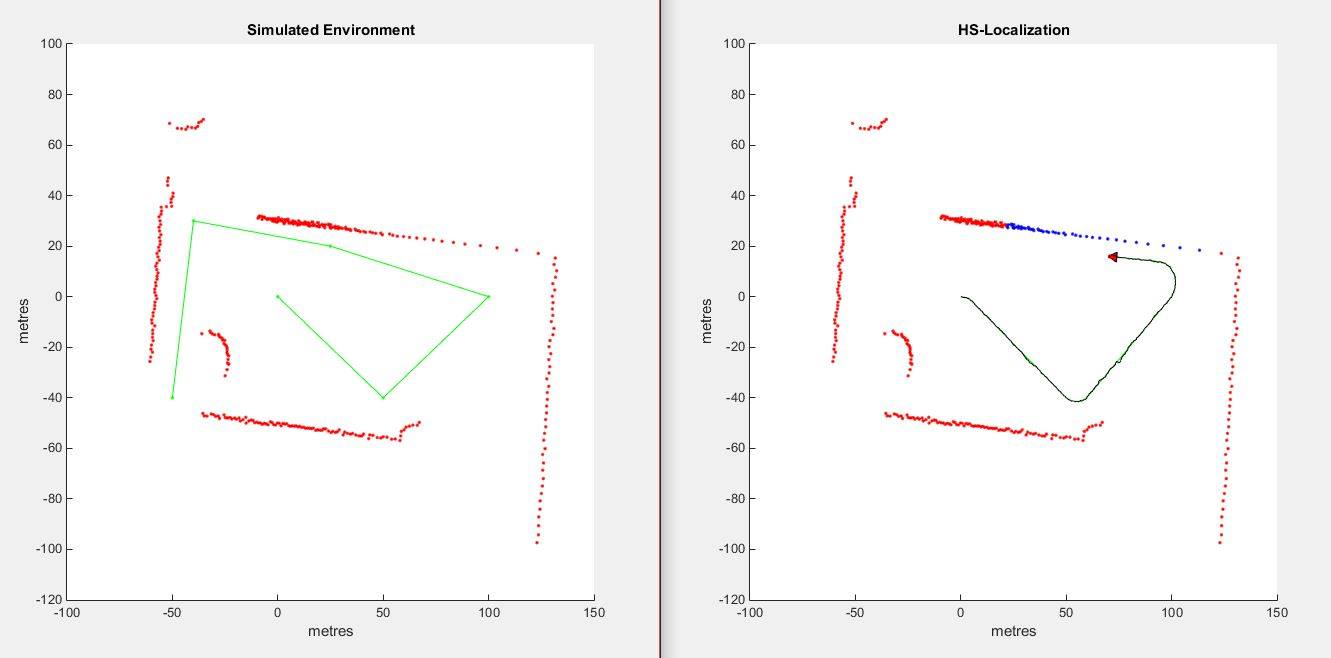
\includegraphics[width=\linewidth]{dataset.jpg}
  \caption{Dataset.}
  \label{fig:dataset}
\end{figure}

\section{METHODOLOGY}
We implemented the following features:
\begin{itemize}
\item Scan-matching using HS and HIDE algorithms.
\item Localization using HS and HIDE algorithms.
\item SLAM using HS algorithm.
\end{itemize}
The parameters are initialized based on experimentations. For scan matching, parameters are chosen to be that given in the paper itself that they obtain after experimenting with different parameters and obtaining the best value. For localization, due to execution speed constraints, we limit some of the parameters to their sub-optimum values. Followinf are the values of the parameters so chosen:\\ $HMS = 30, HMCR = 0.88, NI = 250 \text{ for scan matching } = 20 \text{ for localization }, \lambda = 0.7, F = 0.44,(HRT, NFE) = (14, 220) \text{ for scan matching } = (4, 20) \text{ for localization }$\\ Also from [2], PAR and BW are initialized as follows: \[PAR(t) = PAR_{min}+\frac{PAR_{max}-PAR_{min}}{NI}\times t\] \[bw(t) = bw_{max}e^{\frac{ln(\frac{bw_{min}}{bw_{max}})}{NI}\times t}\] where we choose, $PAR_{min} = 0.55 , PAR_{max}=0.98, bw_{min}=0.2, bw_{max}=8$.\vspace*{1.5mm}\\
\indent Experiments are performed on the dataset explained in section 4. The simulated environment is created using the simulator given by sir for assignment 4. In this simulator, instead of landmarks, scan data is provided as the observations. Input is provided to the vehicle by calculating the inverse of the vehicle transformation matrix and transforming the coordinates of the map to the vehicle's frame of reference. Observations which are within the vehicle range are then returned. This input scan is then matched with the stored map using HS and HIDE algorithms to get the locations of the vehicle. This extimated pose is then passed through the prediction step as in EKF to get the prediction for the next time interval and the above steps are repeated.\vspace*{1mm}\\
\indent To implement slam, we start from an initial map that is the initial observation, assuming that initial pose is known with certainity and then perform localization step as usual in each step. Also in each step, we update the map with the points that are farther than a threshold distance from the already stored map given the position of the robot is known with certain accuracy. This accuracy is measured using the value of the fitting function. In this way we localize our robot while simultaneously mapping the environment.


\section{EXPERIMENTAL RESULTS}
Experiments are perfomed on matlab with the settings explained in section 5. Results obtained from these experiments are shown in fig 2- fig 5. Observations from the results could be summarized as follows:
\begin{itemize}
\item From the scan matching experiments it is observed that both the algorithms are performing quiet well. Also time for execution of 250 iterations of HIDE is 19 sec compared to 250 iterations of HS equal to 7 sec. This is because of the additional DE steps performed after every 14 iterations.
\item Also from figure 4, it is inferred that HIDE converge much faster than HS and that too to the global obtimum. 
\item From figure 5 and 6 it is observed that both the algorithms performed very good with verry less mean squared error. Among both HIDE performed exceptionally well with MSE of X and Y positions almoast ten times less than HS.
\item Time taken by HS to complete its path = 141 sec while that taken by HIDE = 576 sec. Thus HIDE turns out to be much slower, although this time could be improved by reducing HRT and/or NFE, but this will cause degradation of performance.
\item Figure 7 shows that HS SLAM performs as good as HS localization for localization part, but this is only true if continues to get sufficient amount of observations at every time instant, because if at any point of time it don't get bservations, its motion will purely be based on the estimation step, and if considerable error get developed between actual position and estimated position, the subsequent observations will tend to degrade the map and further degrade the localization error.
\item In figure 8, red points represent actual map points while blue points represents estimated map. As we can observe that estimated map is similar to the actual map except for the part in the bottom right corner. This is because the robot never sees that location during its motion, and even if it did, because of such less points in its sight its fitness evaluation comes below the prescribed threshold and it did not update the map.
\end{itemize}
\begin{figure}[H]
  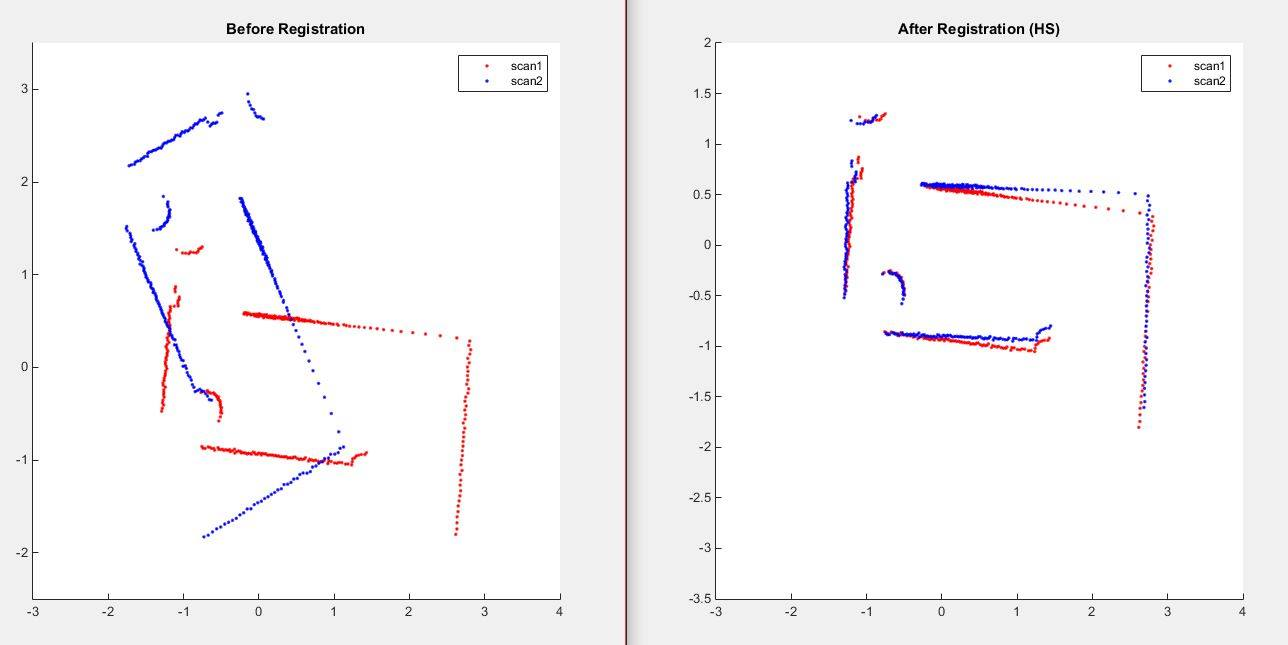
\includegraphics[width=\linewidth]{shs.jpg}
  \caption{Scan Matching with HS}
  \label{fig:dataset}
\end{figure}

\begin{figure}[H]
  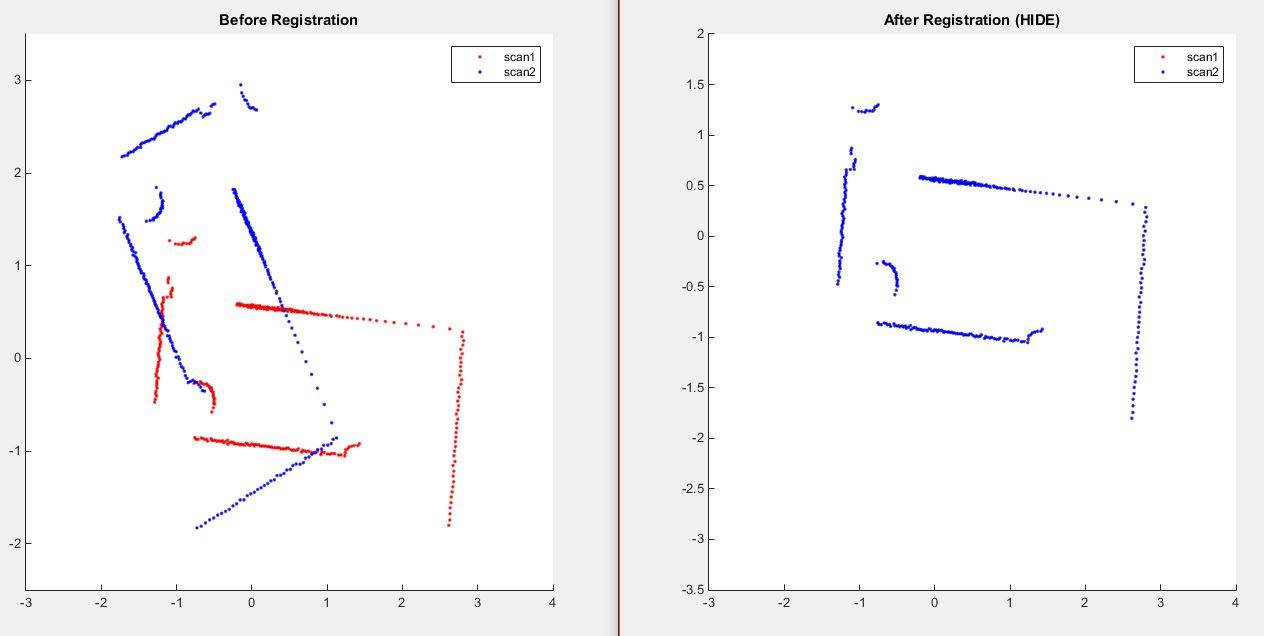
\includegraphics[width=\linewidth]{shide.jpg}
  \caption{Scan Matching with HIDE}
  \label{fig:dataset}
\end{figure}

\begin{figure}[H]
  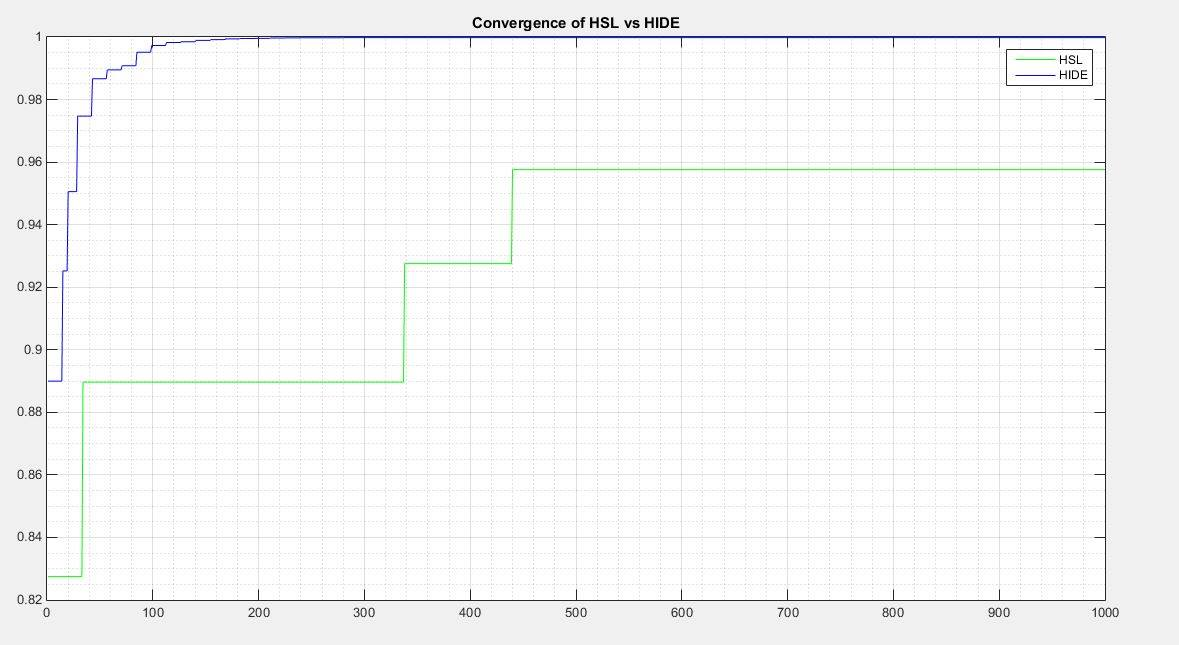
\includegraphics[width=\linewidth]{conv.jpg}
  \caption{Convergence of HS vs HIDE}
  \label{fig:dataset}
\end{figure}

\begin{figure}[H]
  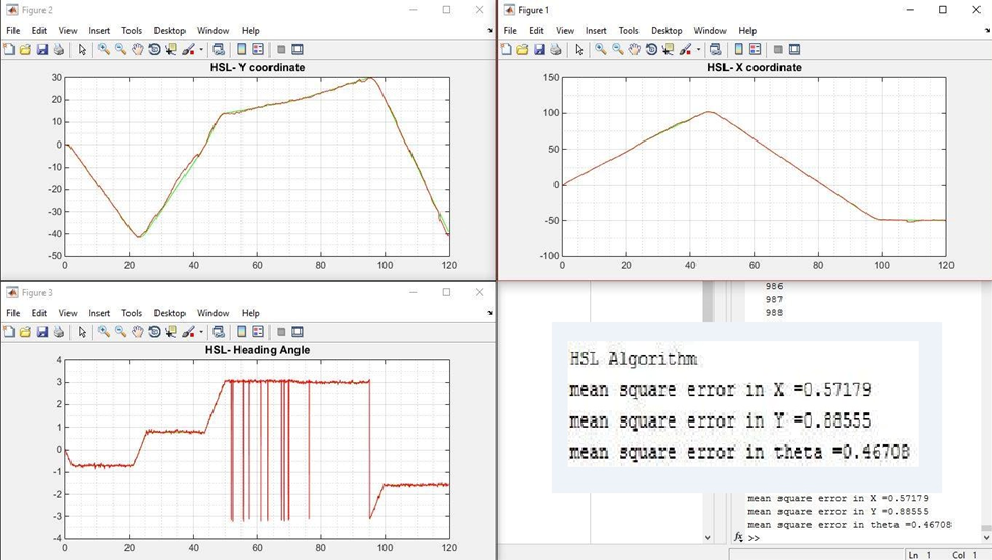
\includegraphics[width=\linewidth]{lhs.png}
  \caption{Localization using HS}
  \label{fig:dataset}
\end{figure}

\begin{figure}[H]
  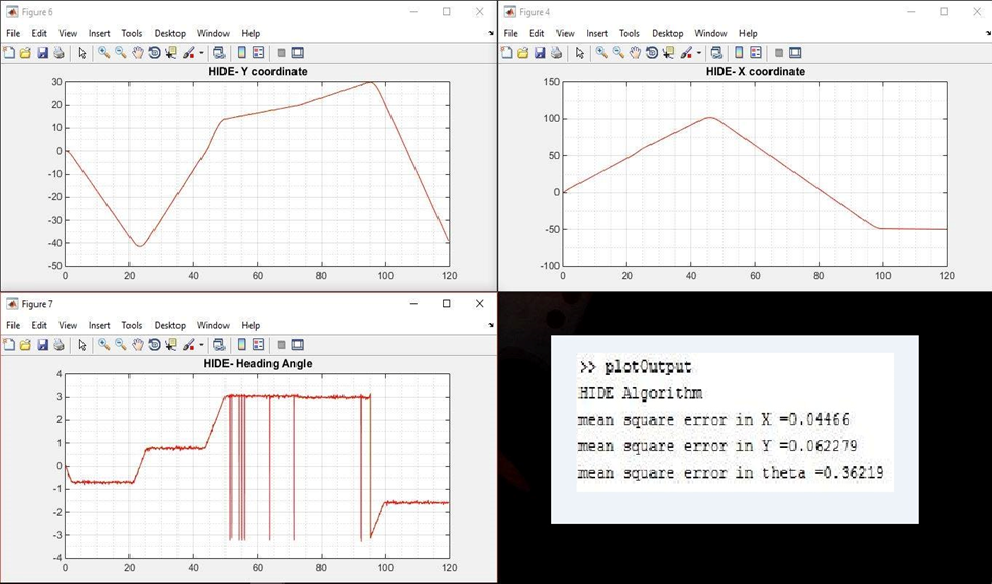
\includegraphics[width=\linewidth]{lhide.png}
  \caption{Localization using HIDE}
  \label{fig:dataset}
\end{figure}

\begin{figure}[H]
  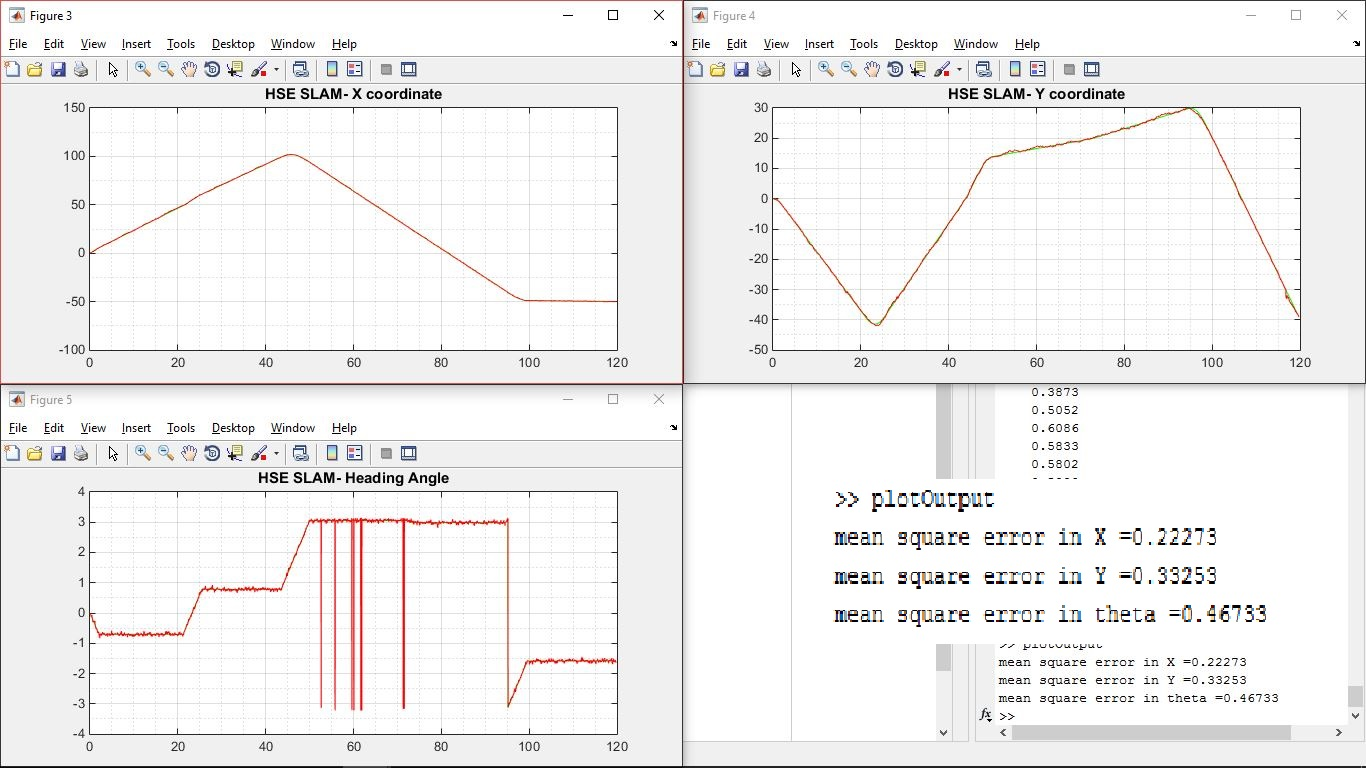
\includegraphics[width=\linewidth]{slam1.jpg}
  \caption{SLAM Localization using HSE}
  \label{fig:dataset}
\end{figure}

\begin{figure}[H]
  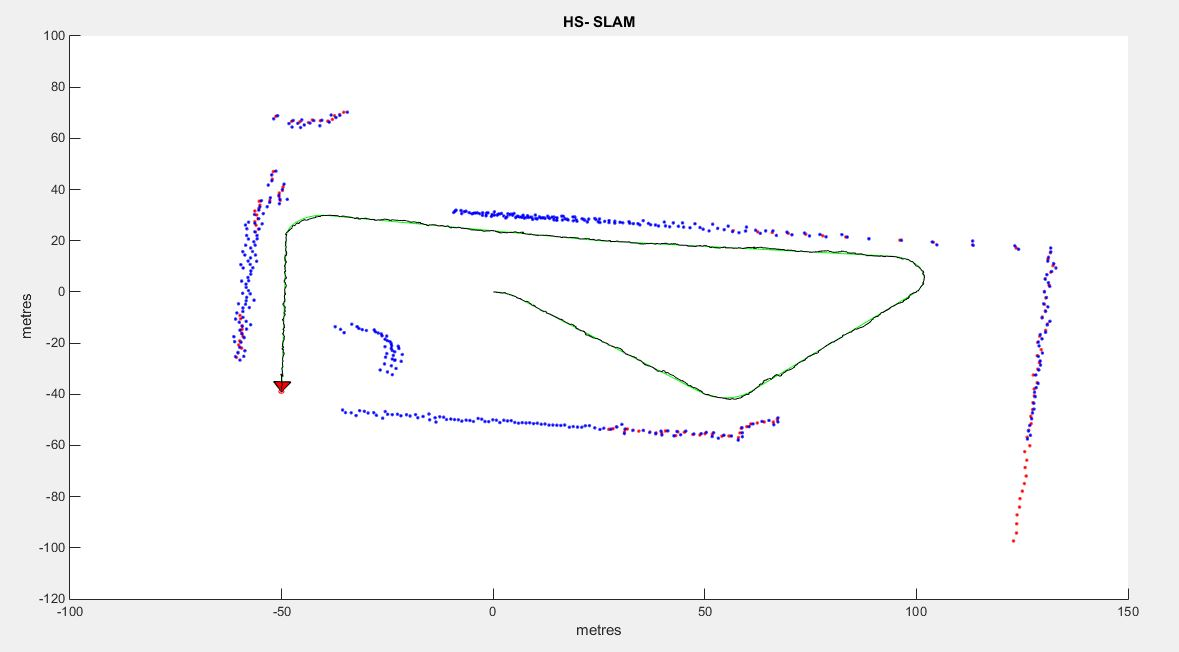
\includegraphics[width=\linewidth]{slam2.jpg}
  \caption{MAP generated through SLAM}
  \label{fig:dataset}
\end{figure}


\section{CONCLUSION}
This project succesfully implemented the scan matching as well as localization algorithms proposed in [1] on the simulated environment and compared their results. The results so obtained agree with what have been obtained by [1]. Additionally we also implemented SLAM using one of the proposed method on the similar simulated environment and obtained satisfactory results. Future work may include proper heuristic developement for SLAM using the above methods, and optimization of the methods to allow for more efficient real time implementations. Also we would like to implement the algorithms on a real system to observe the proposed algorithm's behaviour in real environment.

\section{ACKNOWLEDGMENT}
We would like to Thank Dr. Gaurav Pandey and Mr. N Mohan Krishna for their continuous support throughout the project.

\section{REFERENCES}
[1] Mirkhani, Mohsen, et al. "A novel efficient algorithm for mobile robot localization." Robotics and Autonomous Systems 61.9 (2013): 920-931.\\
\indent [2] Mahdavi, M., Mohammad Fesanghary, and E. Damangir. "An improved harmony search algorithm for solving optimization problems." Applied mathematics and computation 188.2 (2007): 1567-1579.\\
\indent [3] Chakraborty, Uday K., Swagatam Das, and Amit Konar. "Differential evolution with local neighborhood." 2006 IEEE International Conference on Evolutionary Computation. IEEE, 2006.

\end{document}
